\documentclass[11pt,class=report,crop=false]{standalone}
\usepackage[screen]{../python}


\begin{document}


%====================================================================
\chapitre{Algorithmes récursifs}
%====================================================================

\index{recursivite@récursivité}
\index{algorithme recursif@algorithme récursif}

\objectifs{Une fonction récursive est une fonction qui s'appelle elle-même. C'est un concept puissant de l'informatique : certaines tâches compliquées s'obtiennent à l'aide d'une fonction récursive simple. La récursivité est l'analogue de la récurrence mathématique.}


\bigskip


%%%%%%%%%%%%%%%%%%%%%%%%%%%%%%%%%%%%%%%%%%%%%%%%%%%%%%%%%%%%%%%%
%%%%%%%%%%%%%%%%%%%%%%%%%%%%%%%%%%%%%%%%%%%%%%%%%%%%%%%%%%%%%%%%

\begin{cours}[Récursivité (début)]

L'exemple incontournable pour commencer est le calcul des factorielles. On rappelle que 
$$n ! = 1\times 2 \times 3 \times 4 \times \cdots \times (n-1) \times n.$$
\index{factorielle}

Par exemple $5! = 1\times 2 \times 3 \times 4 \times 5 = 120$.


\begin{center}
\begin{minipage}{0.45\textwidth}
\textbf{Algorithme par une boucle.}
\begin{lstlisting}
def factorielle_classique(n):
    f = 1
    for k in range(2,n+1):
        f = f*k
    return f
\end{lstlisting}
\end{minipage}
\begin{minipage}{0.45\textwidth}
\textbf{Algorithme récursif.}
\begin{lstlisting}
def factorielle(n):
    if n == 1:      # Cas terminal
        f = 1
    else:           # Cas général
        f = factorielle(n-1)*n
    return f
\end{lstlisting}
\end{minipage}
\end{center}

L'algorithme classique met en \oe uvre une boucle \og{}pour\fg{} et une variable $f$ qui vaut tour à tour $f=1$, puis $f=1 \times 2$, $f =1 \times 2 \times 3$,\ldots{} jusqu'à $f = 1\times 2 \times 3 \times \cdots \times n = n!$

L'algorithme récursif est différent, regarde bien le code de la fonction \ci{factorielle()} : dans ces lignes de code une instruction fait appel à la fonction \ci{factorielle()} elle-même. L'algorithme est basé sur la relation de récurrence :
$$n! = (n-1)! \times n$$
Donc pour calculer $n!$ il suffit de savoir calculer $(n-1)!$ mais pour calculer $(n-1)!$ il suffit de savoir calculer $(n-2)!$ (car $(n-1)! = (n-2)! \times (n-1)$)\ldots{} Quand-est-ce que cela se termine ?  Lorsque il faut calculer $1!$ alors par définition on sait $1!=1$.


Pour bien comprendre ce qu'il se passe, il est conseillé d'afficher un message à chaque appel de la fonction. Voici une version modifiée de notre fonction récursive:
\begin{center}
%\begin{minipage}{0.45\textwidth}
\begin{lstlisting}
def factorielle(n):
    if n == 1:      # Cas terminal
        print("Cas terminal. Appel de la fonction avec n =",n)
        f = 1
    else:           # Cas général
        print("Cas général.  Appel de la fonction avec n =",n)
        f = factorielle(n-1)*n
    return f
\end{lstlisting}
%\end{minipage}
\end{center} 
La commande \ci{factorielle(10)} renvoie la valeur $10! = 3\,628\,800$. Et au passage voici l'affichage à l'écran produit par cette commande :
\begin{center}
%\begin{minipage}{0.45\textwidth}
\begin{lstlisting}
Cas général.  Appel de la fonction avec n = 10
Cas général.  Appel de la fonction avec n = 9
Cas général.  Appel de la fonction avec n = 8
Cas général.  Appel de la fonction avec n = 7
Cas général.  Appel de la fonction avec n = 6
Cas général.  Appel de la fonction avec n = 5
Cas général.  Appel de la fonction avec n = 4
Cas général.  Appel de la fonction avec n = 3
Cas général.  Appel de la fonction avec n = 2
Cas terminal. Appel de la fonction avec n = 1
\end{lstlisting}
%\end{minipage}
\end{center}

C'est donc un peu comme un compte à rebours, pour calculer $10!$ on demande le calcul de $9!$ qui nécessite le calcul de $8!$\ldots{} lorsque l'on arrive au calcul de $1!$ on renvoie $1$, cela débloque la valeur de $2!$ donc celle de $3!$\ldots{} et à la fin on obtient la valeur de $10!$
\end{cours}

%%%%%%%%%%%%%%%%%%%%%%%%%%%%%%%%%%%%%%%%%%%%%%%%%%%%%%%%%%%%%%%%
%%%%%%%%%%%%%%%%%%%%%%%%%%%%%%%%%%%%%%%%%%%%%%%%%%%%%%%%%%%%%%%%

%\begin{cours}[Récursivité (suite)]
%
%BOF BOF BOF
%
%Voyons une autre fonction récursive.
%On veut déterminer si un entier est ou pas une puissance de $2$. 
%Voici la fonction \ci{est_puissance_2()} qui renvoie \og{}Vrai\fg{} 
%si $n=1,2,4,8,16,32,\ldots$ et \og{}Faux\fg{} sinon.
%
%\begin{center}
%\begin{minipage}{0.45\textwidth}
%\begin{lstlisting}
%def est_puissance_de_2(n):
%    if n == 1:         # Cas terminal
%        return True    # 2^0 = 1 est une puissance de 2
%
%    if n%2 == 0:       # Cas général
%        return est_puissance_de_2(n//2)
%    else:
%        return False   # Cas terminal
%\end{lstlisting}
%\end{minipage}
%\end{center}
%
%Le principe est le suivant pour que $n$ soit une puissance de $2$ il faut que ses seuls diviseurs soit des facteurs $2$. On commence donc par tester si $n$ est pair :
%\begin{itemize}
%  \item si ce n'est pas le cas, c'est terminé $n$ n'est pas une puissance de $2$ ;
%  \item si $n$ est pair, alors on divise $n$ par $2$, et on teste si $n/2$ est une puissance de $2$ par un appel récursif.
%
%\end{cours}




%%%%%%%%%%%%%%%%%%%%%%%%%%%%%%%%%%%%%%%%%%%%%%%%%%%%%%%%%%%%%%%%
% Activité 1 - Pour bien commencer
%%%%%%%%%%%%%%%%%%%%%%%%%%%%%%%%%%%%%%%%%%%%%%%%%%%%%%%%%%%%%%%%

\begin{activite}[Pour bien commencer.]
   
\objectifs{Objectifs : programmer ses premiers algorithmes récursifs.}


\emph{Recommandation.} Comme la récursivité est un concept difficile à appréhender, 
n'hésite pas à afficher les étapes intermédiaires. Par exemple, tu peux commencer chaque fonction par une instruction du type :
\mycenterline{\ci{print("Appel de la fonction avec n =", n)}}

\begin{enumerate}
  \item La somme des carrés des premiers entiers est :
  $$S_n = 1^2 + 2^2 + 3^2 +\cdots + (n-1)^2 + n^2.$$
  
  \begin{enumerate}
    \item Programme une fonction \ci{somme_carres_classique(n)}
    qui calcule cette somme $S_n$ à l'aide d'une boucle.
    
    \item En utilisant la formule de récurrence :
    $$S_1 = 1 \qquad \text{ et } \qquad S_n = S_{n-1} + n^2 \quad \text{ pour } n \ge 2,$$
    programme une fonction \ci{somme_carres(n)} qui calcule $S_n$ par un algorithme récursif.
	Le cas terminal correspond à $n=1$ pour lequel $S_1=1$.
	Le cas général d'un $n \ge 2$, correspond au calcul de la somme $S_n$,
	écrite sous la forme $S_n = S_{n-1} + n^2$. Donc pour calculer $S_{n-1}$ tu effectues un appel récursif à \ci{somme_carres(n-1)}.
  \end{enumerate}	    
     
    
  \item  Programme une fonction récursive \ci{inverser(liste)} qui inverse l'ordre des éléments d'une liste. Par exemple \ci{inverser([1,2,3,4,5])} renvoie \ci{[5,4,3,2,1]}.
  Le principe à suivre est le suivant :
  on extrait le premier élément ; on inverse le reste de la liste ; enfin on rajoute le premier élément à la fin de liste obtenue.
  

\myfigure{1}{\tikzinput{fig_recursivite_1}}  
  
  Voici l'algorithme en détails :
\begin{algorithme}
\sauteligne 
  
\begin{itemize}
  \item 
  \begin{itemize}
   \item Entête : \ci{inverser(liste)}
   \item Entrée : une \ci{liste} $[x_0,x_1,\ldots,x_{n-1}]$ de longueur $n$.
   
   \item Sortie : la liste inversée $[x_{n-1},x_{n-2},\ldots,x_1,x_0]$. 
 
   \item Action : fonction récursive.
  \end{itemize}

   \item \emph{Cas terminal.} Si la longueur $n$ de la liste est $1$ (ou $0$) : renvoyer la liste sans modification (il n'y a rien à inverser).
    
   \item \emph{Cas général.}
    \begin{itemize}
      \item On note $x_0$ le premier élément de \ci{liste}.
      \item On note \ci{fin_liste} le reste de la liste (la liste sans $x_0$).
      \item On effectue un appel récursif \ci{inverser(fin_liste)} qui renvoie une liste \ci{fin_liste_inverse}.
      \item On ajoute à ce résultat l'élément $x_0$ en queue de liste.
      \item On renvoie cette liste.
    \end{itemize}
  \end{itemize}
 \end{algorithme} 
 
 \item Programme une fonction récursive \ci{maximum(liste)} qui renvoie le maximum d'une liste.
 Par exemple \ci{maximum([7,2,9,3,5])} renvoie $9$.
 
 \myfigure{1}{\tikzinput{fig_recursivite_2}}  
  
 
 
 Utilise le principe suivant :
 \begin{itemize}
    \item \emph{Cas terminal.} Si la liste ne contient qu'un seul élément, alors le maximum est cet élément.
    
    \item \emph{Cas général.}
	    \begin{itemize}
	    \item On note $x_0$ le premier élément de la liste.
	    \item On calcule la maximum du reste de la liste par un appel récursif. On note $M'$ ce maximum.
	    \item On compare $x_0$ et $M'$ : si $x_0>M'$ alors on pose $M=x_0$, sinon on pose $M=M'$.
	    \item On renvoie $M$.
		\end{itemize}
  \end{itemize}
    
  \item Programme une fonction récursive \ci{binaire(n)} qui pour un entier $n$ donné, renvoie son écriture binaire sous la forme d'une chaîne de caractères. Par exemple \ci{binaire(23)} renvoie
  \ci{'10111'}.
  
  
  Voici le principe :
  \begin{itemize}
     \item \emph{Cas terminaux.} Si $n=0$ renvoyer \ci{'0'}, si $n=1$ renvoyer \ci{'1'}.
    
    \item \emph{Cas général.}
	    \begin{itemize}
	    \item Calculer l'écriture binaire de $n//2$ par un appel récursif.
	    \item Si $n$ est pair rajouter \ci{'0'} à la fin de la chaîne renvoyée. 
	    \item Sinon rajouter \ci{'1'}.
	    \item Renvoyer la chaîne obtenue.
		\end{itemize}
  \end{itemize}
  
  
\end{enumerate}
 
\end{activite}



%%%%%%%%%%%%%%%%%%%%%%%%%%%%%%%%%%%%%%%%%%%%%%%%%%%%%%%%%%%%%%%%
%%%%%%%%%%%%%%%%%%%%%%%%%%%%%%%%%%%%%%%%%%%%%%%%%%%%%%%%%%%%%%%%

\begin{cours}[Récursivité (suite)]
Voyons un autre exemple de fonction récursive.
On souhaite déterminer si un mot est un palindrome ou pas, c'est-à-dire s'il peut se lire dans les deux sens comme \mot{RADAR} ou \mot{ELLE}.

Voici comment on décide de procéder :
\begin{itemize} 
  \item \emph{Cas terminal numéro 1.} Si le mot contient zéro ou une lettre, c'est un palindrome !
  \item \emph{Cas terminal numéro 2.} Si la première lettre et la dernière lettre sont différentes, alors le mot n'est pas un palindrome (peu importe les lettres du milieu).
  \item \emph{Cas général.} Dans le cas général on sait que le mot contient au moins deux lettres (sinon c'est le cas terminal 1) et que la première et dernière lettre sont identiques (sinon c'est le cas terminal 2). Notre mot est donc un palindrome si et seulement les lettres \og{}du milieu\fg{} forment un palindrome.
\end{itemize}

Voici trois exemples avec la réponse à la question \og{}Est-ce que le mot donné est un palindrome ?\fg{} :
\mycenterline{\mot{RADAR} $\rightarrow$ \mot{ADA} $\rightarrow$ \mot{D} \quad donc \og{}Vrai\fg{}}

\mycenterline{\mot{SERPES} $\rightarrow$ \mot{ERPE} $\rightarrow$ \mot{RP} \quad donc \og{}Faux\fg{}}

\mycenterline{\mot{ELLE} $\rightarrow$ \mot{LL} $\rightarrow$ \mot{"\;"} \quad donc \og{}Vrai\fg{}}

Voici la fonction correspondante :
\begin{center}
%\begin{minipage}{0.45\textwidth}
\begin{lstlisting}
def est_palindrome(mot):
    n = len(mot)
    
    # Cas terminal 1
    if n <= 1:
        return True

    # Cas terminal 2
    if mot[0] != mot[n-1]:
        return False

    # Cas général
    mot_milieu = mot[1:n-1]
    ok_palind = est_palindrome(mot_milieu)    
    return ok_palind
\end{lstlisting}
%\end{minipage}
\end{center}


\end{cours}


%%%%%%%%%%%%%%%%%%%%%%%%%%%%%%%%%%%%%%%%%%%%%%%%%%%%%%%%%%%%%%%%%
%%%%%%%%%%%%%%%%%%%%%%%%%%%%%%%%%%%%%%%%%%%%%%%%%%%%%%%%%%%%%%%%%
%
%\begin{cours}[Récursivité (fin)]
%
%Voici les avantages et les inconvénients de la programmation récursive.
%
%\end{cours}


%%%%%%%%%%%%%%%%%%%%%%%%%%%%%%%%%%%%%%%%%%%%%%%%%%%%%%%%%%%%%%%%
% Activité 2 - Fibonacci et Pascal & Cie
%%%%%%%%%%%%%%%%%%%%%%%%%%%%%%%%%%%%%%%%%%%%%%%%%%%%%%%%%%%%%%%%

\begin{activite}[Fibonacci, Pascal \& Cie]
   
\objectifs{Objectifs : étudier des cas de récursivité plus compliqués.}

\begin{enumerate}
  \item \textbf{Fibonacci.}
  \index{suite!de Fibonacci}
  
  La suite de Fibonacci est définie par une formule de récurrence qui dépend des deux termes précédents.
  $$F_0 = 0 \quad\text{ et }\quad  F_1 = 1 \qquad \text{ puis } \quad F_{n} = F_{n-1} + F_{n-2} \quad \text{ pour } n\ge2.$$
  Vérifie que les premiers termes sont :
  $$F_0 = 0 \quad F_1 = 1 \quad F_2 = 1 \quad F_3 = 2 \quad F_4 = 3 \quad F_5 = 5  \quad F_6 = 8 \quad \ldots$$
  
  Programme une fonction récursive \ci{fibonacci(n)} qui renvoie $F_n$.
  \begin{itemize}
    \item Les cas terminaux sont pour $n=0$ et $n=1$.
    \item Pour le cas général, il faut faire deux appels récursifs : un appel de la fonction au rang $n-1$ qui renvoie $F_{n-1}$ et un appel au rang $n-2$ qui renvoie $F_{n-2}$. Ensuite tu renvoies la somme de ces deux nombres.
  \end{itemize}
    
   
  \emph{Commentaires.} Cet algorithme n'est pas efficace car il est très lent pour  $n\ge 30$. Essaie de comprendre pourquoi. Pour répondre à cette question tu peux afficher \og{}Tiens, je calcule encore $F_2$ !\fg{} à chaque appel de la fonction pour lequel $n=2$. 
  
    
  \item \textbf{Coefficients du binôme.}
  \index{coefficients du binome de Newton@coefficients du binôme de Newton}
  
  Les \defi{coefficients du binôme de Newton} $C_{k,n}$  sont définis pour $0 \le k \le n$.
  Ils se calculent par une formule de récurrence :
  
  $$C_{k,n} = 
  \begin{cases}
  1 & \text{ si } k=0 \text{ ou } k=n \\
  C_{k-1,n-1} + C_{k,n-1} & \text{ sinon.}
  \end{cases}$$
  
  Un coefficient s'obtient donc comme la somme de deux autres.
  Ce coefficient $C_{k,n}$ est habituellement noté $\binom{n}{k}$ et lu \og{}$k$ parmi $n$\fg{}.
  
   \myfigure{1}{\tikzinput{fig_recursivite_4}}  
  

Ce sont aussi les coefficients qui apparaissent dans le développement de $(a+b)^n$.  
Par exemple :
$$(a+b)^4 = a^4 + {\color{red}4}a^3b + {\color{red}6}a^2b^2 + {\color{red}4}ab^3 + b^4$$
et on a 
$$C_{0,4} = 1 \qquad  C_{1,4} = {\color{red}4} \qquad C_{2,4} = {\color{red}6} \qquad C_{3,4} = {\color{red}4} \qquad C_{4,4} = 1$$
  
  Programme une fonction récursive \ci{binome(k,n)} qui renvoie $C_{k,n}$.
  \begin{itemize}
    \item Les cas terminaux sont pour $k=0$ et $k=n$.
    \item Pour le cas général, il faut faire deux appels récursifs : un appel pour $C_{k-1,n-1}$ et un autre pour $C_{k,n-1}$.
  \end{itemize}
  
  \item \textbf{Triangle de Pascal.}
  \index{triangle de Pascal}
  
  Utilise ta fonction précédente pour afficher le \defi{triangle de Pascal} :
  la ligne numéro $n$ est composée des coefficients $C_{k,n}$ pour $k=0,1,\ldots,n$ (la numérotation $n$ des lignes commence avec $n=0$).

Sur la figure de gauche le principe du calcul du triangle de Pascal : le triangle se remplit ligne par ligne, chaque nombre étant la somme issue des deux flèches qui y arrivent. Sur la figure de droite la sortie à l'écran attendue.

\begin{center} 
\begin{minipage}{0.4\textwidth}   
\myfigure{0.8}{\tikzinput{fig_recursivite_5}}  
 \end{minipage}\quad
\begin{minipage}{0.5\textwidth} 
\begin{lstlisting}
1 
1 1 
1 2 1 
1 3 3 1 
1 4 6 4 1 
1 5 10 10 5 1 
1 6 15 20 15 6 1 
1 7 21 35 35 21 7 1 
1 8 28 56 70 56 28 8 1 
1 9 36 84 126 126 84 36 9 1 
1 10 45 120 210 252 210 120 45 10 1
\end{lstlisting}
\end{minipage}
\end{center} 
  
  \emph{Indications.} Voici comment afficher une chaîne de caractères à l'écran sans passer à la ligne suivante : \ci{print(chaine,end="")}.
  
   \item \textbf{Triangle de Pascal des termes impairs.}
   Modifie ta fonction précédente de façon à afficher un \ci{"X"} à la place d'un terme $C_{k,n}$ impair et une espace pour un terme pair.
   Quelle figure géométrique reconnais-tu ?
   
\begin{center} 
\begin{minipage}{0.2\textwidth} 
\begin{lstlisting}
X
XX
X X
XXXX
X   X
XX  XX
X X X X
XXXXXXXX
X       X
XX      XX
X X     X X
\end{lstlisting}
\end{minipage}
\end{center} 


   
   \item \textbf{Somme des chiffres.} Programme une fonction récursive \ci{somme_chiffres(n)}
   qui calcule la somme des chiffres qui composent l'entier $n$. Par exemple
   avec $n = 1\,357\,869$, la fonction renvoie $n' = 39$.
   
   Pour cela sépare l'entier $n$ en deux parties : 
   \begin{itemize}
     \item le chiffre des unités, obtenu par $n\%10$ (sur l'exemple $n\%10=9$),
     \item la partie restante de l'écriture décimale de l'entier, obtenue par $n//10$  (sur l'exemple $n//10 = 135\,786$).
   \end{itemize}
   
   \item \textbf{Résidu d'un entier.} 
   L'entier $n = 1\,357\,869$ sera divisible par $3$, si et seulement si sa somme de chiffres $n'=39$
   est divisible par $3$. Comment savoir si $n'$ est divisible par $3$ ? On recommence en calculant la somme des chiffres de $n'$, ici on obtient $n''=12$. Comment savoir si $n''$ est divisible par $3$ ? La somme des chiffres est $n'''=3$ qui est bien divisible par $3$. Donc $n''$, $n'$ et $n$ sont divisibles par $3$. 
   
   Le \defi{résidu} d'un entier $n$ est l'entier $r$ compris entre $0$ et $9$ obtenu en itérant le processus : prendre la somme des chiffres et recommencer. Ainsi le résidu de $n = 1\,357\,869$ est $r=3$.
   
   Programme une fonction récursive \ci{residu_chiffres(n)} qui calcule le résidu $r$ de l'entier $n$.
   
   \emph{Indications.} La fonction \ci{residu_chiffres()} fait d'abord appel à la fonction précédente 
   \ci{somme_chiffres()} puis fait un appel récursif.
\end{enumerate}

\end{activite}


%%%%%%%%%%%%%%%%%%%%%%%%%%%%%%%%%%%%%%%%%%%%%%%%%%%%%%%%%%%%%%%%
%%%%%%%%%%%%%%%%%%%%%%%%%%%%%%%%%%%%%%%%%%%%%%%%%%%%%%%%%%%%%%%%

\begin{cours}[Parcours d'arbre]

\textbf{Arbre.}\index{arbre}
On souhaite construire toutes les listes possibles de $n$ éléments formées avec les trois choix $0,1,2$.
\begin{itemize}
  \item Si $n=1$, il n'y a que trois listes possibles d'un seul élément chacune : $[0]$, $[1]$, $[2]$. 
   \item Si $n=2$, il n'y a que $9$ listes possibles ayant deux éléments : $[0, 0]$,  $[0, 1]$, $[0, 2]$, $[1, 0]$, $[1, 1]$, $[1, 2]$, $[2, 0]$, $[2, 1]$, $[2, 2]$. 
   \item On modélise cela sous la forme d'un arbre : les arêtes sont les choix $0$, $1$ ou $2$. Les sommets sont les listes obtenues.
   
\begin{minipage}{0.35\textwidth}   
\myfigure{0.7}{\tikzinput{fig_recursivite_8}}
\end{minipage}
\begin{minipage}{0.59\textwidth}  
\myfigure{0.9}{\tikzinput{fig_recursivite_7}}
\end{minipage}

\medskip

  \item Pour le cas général, il y a $3^n$ listes. Si on regarde l'arbre du haut vers le bas, alors on descend d'un sommet en rajoutant $0$, $1$ ou $2$ \emph{à la fin} de la liste.
   
\myfigure{1}{\tikzinput{fig_recursivite_6}}  
\end{itemize}

\medskip


\textbf{Algorithme récursif.}

L'idée récursive pour construire toutes ces listes est la suivante :
\begin{itemize}
  \item on suppose que l'on a construit toutes les listes possibles de longueur $n-1$, 
  \item on ajoute $0$ \emph{en tête} de chacune de ces listes,
  \item puis on ajoute $1$ \emph{en tête} de chacune de ces listes,
  \item enfin on ajoute $2$  \emph{en tête} de chacune de ces listes.
  \item On obtient donc $3$ fois plus de listes qu'au départ.
  \item En terme d'arbre : pour construire l'arbre $\mathcal{A}_n$, on part de trois copies de l'arbre $\mathcal{A}_{n-1}$ reliées par un même sommet au-dessus avec des arêtes pondérées par $0$, $1$ et $2$.

\smallskip

\myfigure{1}{\tikzinput{fig_recursivite_9}}  
\end{itemize}

\textbf{Fonction.}

Voici la fonction \ci{parcours(n)} qui renvoie toutes les listes possibles ayant $n$ éléments.

\begin{lstlisting}
def parcours(n):
    # Cas terminal
    if n == 1:
        return [[0],[1],[2]]    # ou bien n == 0 il faut [[]]

    # Cas général
    sous_liste = parcours(n-1)  
    liste_deb_0 = [ [0] + x for x in sous_liste ]
    liste_deb_1 = [ [1] + x for x in sous_liste ]
    liste_deb_2 = [ [2] + x for x in sous_liste ]
    liste = liste_deb_0 + liste_deb_1 + liste_deb_2
    return liste
\end{lstlisting}


\begin{itemize}
  \item Pour $n=1$, la fonction renvoie la liste $[[0], [1], [2]]$.
  \item Pour $n=2$, il y a $3^2=9$ éléments : $[[0, 0], [0, 1], [0, 2], [1, 0], [1, 1], [1, 2], [2, 0], [2, 1], [2, 2]]$.
  \item Pour $n=3$, il y a $3^3=27$ éléments : $[[0, 0, 0], [0, 0, 1], [0, 0, 2], [0, 1, 0], [0, 1, 1], \ldots, [2, 2, 1], [2, 2, 2]]$.
\end{itemize}

\end{cours}


%%%%%%%%%%%%%%%%%%%%%%%%%%%%%%%%%%%%%%%%%%%%%%%%%%%%%%%%%%%%%%%%
% Activité 3 - Parcours d'arbre
%%%%%%%%%%%%%%%%%%%%%%%%%%%%%%%%%%%%%%%%%%%%%%%%%%%%%%%%%%%%%%%%

\begin{activite}[Parcours d'arbre]
   
\objectifs{Objectifs : résoudre des problèmes en parcourant des arbres.}

\begin{enumerate}
  \item \textbf{Pile ou face.}
  
  Programme une fonction \ci{pile_ou_face(n)} qui renvoie la liste de tous les tirages possibles à pile ou face avec $n$ lancers.
  Par exemple :
  \begin{itemize}
    \item pour $n=1$ (cas terminal), la fonction renvoie \ci{['P','F']} (soit pile, soit face) ;
    \item pour $n=2$, elle renvoie \ci{['PP','PF','FP','FF']} (premier tirage pile/pile, \ldots) ;
    \item pour $n=3$ : \ci{['PPP','PPF','PFP','PFF','FPP','FPF','FFP','FFF']}.
  \end{itemize}
  
  \emph{Indications.} Base-toi sur le modèle de parcours d'arbre du cours ci-dessus avec ici deux choix au lieu de trois.
  
  \myfigure{0.7}{\tikzinput{fig_recursivite_10}} 

  \item \textbf{Réduire des listes emboîtées.}
  
  On considère une liste qui peut contenir des entiers, ou bien des listes d'entiers, ou bien des listes contenant des entiers et des listes d'entiers\ldots
  
  Par exemple :
  \mycenterline{\ci{[ [1,2], 3, [9,8,7,[6,5]], [[1],[2,3]] ]}}
  
  On veut en extraire les éléments atomiques (les entiers) : 
  \mycenterline{\ci{[1, 2, 3, 9, 8, 7, 6, 5, 1, 2, 3]}}
  
  Voici comment modéliser les imbrications sous forme d'un arbre : les sommets sont soit des entiers, soit des listes. Pour les sommets qui sont des listes ses enfants sont les éléments de cette liste.

  \myfigure{0.7}{\tikzinput{fig_recursivite_11}} 

  Programme une fonction \ci{une_seule_liste(liste)} qui effectue la tâche demandée.
  C'est assez simple avec un algorithme récursif. 
  \begin{itemize} 
    \item Définir une liste des éléments extraits qui au départ est une liste vide.
    \item Pour chaque élément de la liste :
  \begin{itemize}
    \item soit c'est un entier (cas terminal) et on l'ajoute à la liste des éléments extraits,
    \item soit c'est une liste (cas général) et par un appel récursif on en extrait ses éléments. On ajoute ces éléments à la liste des éléments extraits. 
  \end{itemize}
    \item Renvoyer la liste des éléments extraits.
    
  \end{itemize}
  
  \bigskip
  
  \emph{Indications.} Pour savoir si un élément est un entier ou bien une liste, tu peux utiliser la fonction \ci{isinstance(element,type)}.\index{isinstance@\ci{isinstance}} Par exemple :
  \begin{itemize}
    \item \ci{isinstance(5,int)} renvoie \og{}Vrai\fg{},
    \item \ci{isinstance(7,list)} renvoie \og{}Faux\fg{}.
  \end{itemize}

  \bigskip
    
  \emph{Challenge.} Essaie de programmer cette fonction sans la récursivité ! 
  

  
\end{enumerate}


\emph{Tu trouveras une très belle application de parcours d'arbres dans la fiche \og{}Le compte est bon\fg{}.}
 
\end{activite}



%%%%%%%%%%%%%%%%%%%%%%%%%%%%%%%%%%%%%%%%%%%%%%%%%%%%%%%%%%%%%%%%
% Activité 4 - Diviser pour régner
%%%%%%%%%%%%%%%%%%%%%%%%%%%%%%%%%%%%%%%%%%%%%%%%%%%%%%%%%%%%%%%%

\begin{activite}[Diviser pour régner]
   
\objectifs{Objectifs : séparer un problème en deux morceaux et traiter chaque morceau de façon récursive.}

\begin{enumerate}
  \item \textbf{Minimum.}
  
  Programme une fonction récursive \ci{minimum(liste)} qui renvoie le minimum d'une liste de nombres.
  Par exemple avec la liste $[7,5,3,9,1,12,13]$ la fonction renvoie $1$.
  
  L'idée est de séparer la liste en une partie gauche et une partie droite. 
  \begin{itemize}
    \item On traite chaque partie séparément : un appel récursif renvoie le minimum de la sous-liste de gauche et un appel récursif renvoie le minimum de la sous-liste de droite. 
     
    \item Le minimum de la liste est donc le plus petit de ces deux minimums.
    
    \item Le cas terminal est lorsque la liste est de longueur $1$.
  \end{itemize}
    
  \item \textbf{Distance de Hamming.} 
  
  La \defi{distance de Hamming} entre deux listes de même longueur est le nombre de rangs pour lesquels éléments sont différents.
  Par exemple les listes $[1,2,3,4,5,6,7]$ et $[1,2,0,4,5,0,7]$ diffèrent à deux endroits, donc la distance de Hamming entre les deux listes vaut $2$.
  
  Programme une fonction récursive \ci{distance_hamming(liste1,liste2)}.
  
  Réfléchis au cas terminal (la longueur de la liste est $1$) et à comment calculer la distance de Hamming entre deux listes connaissant la distance entre les demi-listes à gauche et la distance entre les demi-listes à droites.
  
  \item \textbf{Factorielle (encore !).}
	\index{factorielle}
  
  Soient $a$ et $b$ deux entiers avec $b>0$. 
  On définit une généralisation de la factorielle :
  $$p(a,b) = a(a+1)(a+2)\cdots (b-2)(b-1)$$
  (il y a $b-a$ facteurs).
  
  Par exemple $p(10,16) = 10 \times 11 \times 12 \times 13 \times 14 \times 15$.
  
  On se propose de calculer $p(a,b)$ par la formule :
  $$p(a,b) = p(a,a+k//2) \cdot p(a+k//2,b) \qquad \text{ où } k = b-a.$$
  Sur notre exemple cela revient à décomposer le produit en deux sous-produits :
  $$p(10,16) = \big(10 \times 11 \times 12\big) \times \big(13 \times 14 \times 15\big) = p(10,13) \times p(13,16).$$
  
  
  Transforme cette formule en un algorithme récursif et en une fonction récursive \ci{produit(a,b)}.
  
  Utilise ceci pour obtenir une nouvelle méthode de calcul de $n!$
  
  
  
\end{enumerate}
 
\end{activite}



%%%%%%%%%%%%%%%%%%%%%%%%%%%%%%%%%%%%%%%%%%%%%%%%%%%%%%%%%%%%%%%%
%%%%%%%%%%%%%%%%%%%%%%%%%%%%%%%%%%%%%%%%%%%%%%%%%%%%%%%%%%%%%%%%

\begin{cours}[Dérangements]


Des couples arrivent à un bal masqué, chaque couple est déguisé en une paire de \emph{Wonderwoman}/\emph{Superman}. Lors de la fête les couples sont séparés et les danseurs se mélangent. Au moment du bal chaque \emph{Wonderwoman} danse avec un \emph{Superman}. Quelle est la probabilité qu'aucun de ces couples de danseurs soit un couple initial ?

\myfigure{0.5}{\tikzinput{fig_derangement_7}}  

\textbf{Permutation.}
On numérote les \emph{Wonderwoman} de $0$ à $n-1$ et on attribue le même numéro $i$
au \emph{Superman} en couple avec la \emph{Wonderwoman} numéro $i$.

Pendant le bal les couples se reforment et la \emph{Wonderwoman} numéro $i$ danse avec n'importe lequel des \emph{Superman} du numéro $0$ jusqu'au numéro $n-1$ (y compris son légitime numéro $i$).
On note ce couple $i \mapsto j$.

\myfigure{0.5}{\tikzinput{fig_derangement_8}}  

\textbf{Permutation et dérangement.}

\begin{itemize}
    \item Une \defi{permutation}\index{permutation} est une liste d'associations $i \mapsto j$, pour $i,j$ dans $\{0,\ldots,n-1\}$.
    \item Le nombre de permutations possibles est $n!$ 
    \item Un exemple avec $n=3$ : voici les $3!=6$ permutations possibles :
\myfigure{0.8}{\tikzinput{fig_derangement_6}}      


    \item Voici deux exemples avec $n=5$ :
\myfigure{0.6}{\tikzinput{fig_derangement_5}}     
    
    \item Un \defi{dérangement} est une permutation qui vérifie $i\neq j$, pour l'association $i \mapsto j$ et ce quel que soit $i=0,\ldots,n-1$.
    \item Voici la liste des dérangements pour $n=3$ : 
\myfigure{0.6}{\tikzinput{fig_derangement_3}}    
       
    \item Les autres permutations pour $n=3$ ne sont pas des dérangements, par exemple la permutation suivante vérifie $1 \mapsto 1$ donc n'est pas un dérangement :
 \myfigure{0.6}{\tikzinput{fig_derangement_4}}    
 
   \item Pour les deux permutations d'ordre $n=5$ définies en exemple ci-dessus, l'une est un dérangement et l'autre pas. Trouve qui est qui.

\end{itemize}
   
   
   
\textbf{Modélisation.}
On modélise une permutation par la liste des images :
\myfigure{0.7}{\tikzinput{fig_derangement_2}}

Une permutation d'ordre $n$ sera donc représentée par une liste dans laquelle les entiers de $0$ à $n-1$ apparaissent chacun une fois et une seule.
Voici un exemple de permutation d'ordre $5$ et sa représentation par une liste :
\myfigure{0.7}{\tikzinput{fig_derangement_1}}

\end{cours}



%%%%%%%%%%%%%%%%%%%%%%%%%%%%%%%%%%%%%%%%%%%%%%%%%%%%%%%%%%%%%%%%
% Activité 5 - Dérangements
%%%%%%%%%%%%%%%%%%%%%%%%%%%%%%%%%%%%%%%%%%%%%%%%%%%%%%%%%%%%%%%%

\begin{activite}[Dérangements]
   
\objectifs{Objectifs : calculer le nombre de dérangements par différentes méthodes.}


\objectifs{Rappel du problème : Des couples arrivent à un bal masqué, chaque couple est déguisé en une paire de \emph{Wonderwoman}/\emph{Superman}. Lors de la fête les couples sont séparés et les danseurs se mélangent. Au moment du bal chaque \emph{Wonderwoman} danse avec un \emph{Superman}. Quelle est la probabilité qu'aucun de ces couples de danseurs ne soit un couple initial ?}

Le \defi{nombre de dérangements} $d_n$ est défini par :
$$d_1 = 1 \qquad \text{ et } \qquad d_n = nd_{n-1} + (-1)^n \quad \text{ pour } n\ge2.$$
\begin{enumerate}
  \item Programme une fonction \ci{derangement_classique(n)} qui renvoie $d_n$ en utilisant une boucle.
  
  \emph{Indications.} $(-1)^n = + 1$ si $n$ est pair et $-1$ sinon.
    
  \item Programme une fonction récursive \ci{derangement(n)} qui renvoie aussi $d_n$.
  
  \item La probabilité qu'aucun des couples initiaux ne soit reformé est donnée par :
  $$p_n = \frac{d_n}{n!}.$$

   \begin{itemize}
     \item Calcule cette probabilité pour de petites valeurs de $n$.   
     \item Compare cette probabilité avec $1/e$ (où $e=\exp(1)=2.718\ldots$). 
     \item Est-ce que la convergence est rapide (quand $n\to+\infty$) ?
     \item Conclure : \og{}Il y a environ \ \ldots\ldots{} \%{} de chance qu'aucun couple initial ne soit reformé.\fg{}
    \end{itemize}
   
   \item \textbf{Dérangement ?} 
   
   On se donne une permutation sous la forme d'une liste d'entiers de $0$ à $n-1$.
   Programme une fonction \ci{est_derangement(permutation)} qui teste si la permutation donnée est (ou pas) un dérangement.
   
   \emph{Dérangement.} On rappelle que pour un dérangement on n'a jamais $i \mapsto i$. 
   
   \emph{Exemple.} La permutation codée par $[2,0,3,1]$ est un dérangement, la fonction renvoie \og{}Vrai\fg{}. Par contre la permutation codée par $[3,1,2,0]$ n'est pas un dérangement, car $2 \mapsto 2$, la fonction renvoie \og{}Faux\fg{}.
   
   \item \textbf{Toutes les permutations.}
   
   Programme une fonction \ci{toutes_permutations(n)} qui renvoie la liste de toutes les permutations de longueur $n$.
   
   Par exemple pour $n=3$, voici la liste de toutes les permutations possibles :  
   \mycenterline{\ci{[[2, 1, 0], [1, 2, 0], [1, 0, 2], [2, 0, 1], [0, 2, 1], [0, 1, 2]]}}
   
   Pour cela l'algorithme est basé sur un principe récursif : par exemple si on connaît toutes les permutations à trois éléments (voir juste au-dessus), alors on obtient les permutations à $4$ éléments en insérant la valeur $3$ à toutes les positions possibles de toutes les permutations à $3$ éléments possibles :
\begin{itemize}
  \item notre première permutation à trois éléments $[2,1,0]$, donne par insertion de $3$ les permutations à quatre éléments $[3,2,1,0]$, $[2,3,1,0]$, $[2,1,3,0]$ et $[2,1,0,3]$ ;
  \item ensuite avec $[1,2,0]$ on obtient $[3,1,2,0]$, $[1,3,2,0]$, $[1,2,3,0]$, $[1,2,0,3]$ ;
  \item on continue avec les autres permutations pour obtenir en tout $4! = 24$ permutations d'ordre $4$.
\end{itemize}
   
  \begin{algorithme}
\sauteligne 
  
\begin{itemize}
  \item 
  \begin{itemize}
   \item Entête : \ci{toutes_permutations(n)}
   \item Entrée : un entier $n$.
   \item Sortie : la liste des $n!$ permutations d'ordre $n$.
   \item Action : fonction récursive.
  \end{itemize}

   \item \emph{Cas terminal.} Si $n=1$ alors renvoyer la liste \ci{[ [0] ]} (qui contient l'unique permutation à un seul élément).
    
   \item \emph{Cas général.}
    \begin{itemize}      
      \item On effectue un appel récursif \ci{toutes_permutations(n-1)} qui renvoie une liste \ci{old_liste} de permutations d'ordre $n-1$.
      \item Une \ci{new_liste} est initialisée à la liste vide.
      
      \item Pour chaque permutation de \ci{old_liste} et pour chaque $i$ allant de $0$ à $n-1$, on insère le nouvel élément $n-1$ au rang $i$. On ajoute cette nouvelle permutation d'ordre $n$ à \ci{new_liste}.

      \item On renvoie \ci{new_liste}.
    \end{itemize}
  \end{itemize}
 \end{algorithme} 
 
 \item \textbf{Tous les dérangements.}
 
 Programme une fonction \ci{tous_derangements(n)} qui à partir de la liste de toutes les permutations d'ordre $n$ ne renvoie que les dérangements. 
 Vérifie sur les premières valeurs de $n$ que ce nombre de dérangements vaut bien $d_n$.
  
\end{enumerate}

\end{activite}


%%%%%%%%%%%%%%%%%%%%%%%%%%%%%%%%%%%%%%%%%%%%%%%%%%%%%%%%%%%%%%%%
%%%%%%%%%%%%%%%%%%%%%%%%%%%%%%%%%%%%%%%%%%%%%%%%%%%%%%%%%%%%%%%%

\begin{cours}[Tortue \Python]

Voici un bref rappel des principales fonctions du module \ci{turtle} afin de diriger la tortue de \Python :

\begin{itemize}
  \item \ci{forward(100)}/\ci{backward(100)}  avancer/reculer de $100$ pixels, 
  \item \ci{left(90)}/\ci{right(90)} tourner à gauche/droite de $90$ degrés, 
  \item \ci{goto(x,y)} aller à la position $(x,y)$,
  \item \ci{x,y = position()} récupérer les coordonnées courantes de la tortue, 
  \item \ci{setheading(angle)} s'orienter dans la direction donnée,
  \item \ci{up()}/\ci{down()} lever/abaisser le stylo,
  \item \ci{width(3)}, \ci{color('red')} style du tracé,
  \item \ci{showturtle()}/\ci{hideturtle()} affiche/cache le pointeur,
  \item \ci{speed('fastest')} pour aller plus vite,
  \item \ci{exitonclick()} à placer à la fin.
\end{itemize}

\end{cours}

%%%%%%%%%%%%%%%%%%%%%%%%%%%%%%%%%%%%%%%%%%%%%%%%%%%%%%%%%%%%%%%%
% Activité 6 - Tortue récursive
%%%%%%%%%%%%%%%%%%%%%%%%%%%%%%%%%%%%%%%%%%%%%%%%%%%%%%%%%%%%%%%%

\begin{activite}[Tortue récursive]

\index{tortue}   

\objectifs{Objectifs : tracer des fractales à l'aide de la tortue et des algorithmes récursifs.}

\begin{enumerate}
  \item \textbf{Le flocon de Koch.}
  \index{fractale!flocon de Koch}
  
  Le flocon de Koch est une fractale définie par un processus récursif.
  \`A chaque étape, chaque segment est remplacé par $4$ nouveaux segments plus petits formant une dent. Voici les étapes en partant d'un segment horizontal.
  
  \bigskip
  

\myfigure{1}{\tikzinput{fig_koch}}

%\begin{center}
%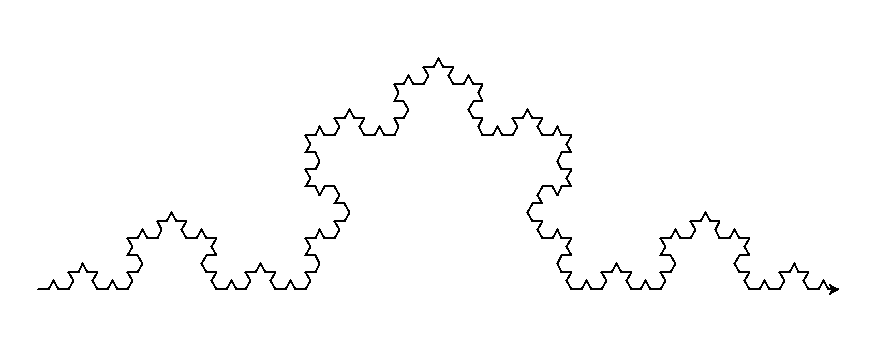
\includegraphics[scale=0.14]{ecran_tortue_koch}
%\end{center}
   
   Définis une fonction récursive \ci{koch(l,n)} qui trace le flocon de Koch d'ordre $n$ ;
   $\ell$ est un paramètre de longueur.
   
   Le principe du tracé est le suivant :
   \begin{itemize}
     \item \emph{Cas terminal.} Si $n=0$, tracer un segment de longueur $\ell$.
     
     \item \emph{Cas général.}
     \begin{itemize}  
       \item Tracer le flocon de Koch d'ordre $n-1$, associé à la longueur $\ell/3$.
       \item Tourner un peu vers la gauche.
       \item Tracer le flocon de Koch d'ordre $n-1$, associé à la longueur $\ell/3$.
       \item Tourner vers la droite.
       \item Tracer le flocon de Koch d'ordre $n-1$, associé à la longueur $\ell/3$.       
       \item Tourner un peu vers la gauche.
       \item Tracer le flocon de Koch d'ordre $n-1$, associé à la longueur $\ell/3$.
     \end{itemize}       
  \end{itemize}    
    
  \item  \textbf{Arbre binaire.} 
  
  Adapte la fonction précédente en une fonction \ci{arbre(l,n)} pour dessiner des arbres dont la profondeur dépend d'un paramètre $n$ ($\ell$ est un paramètre de longueur).
  
  Voici les dessins pour $n=1$, $n=2$, $n=3$ et $n=6$.
  
  \begin{center}
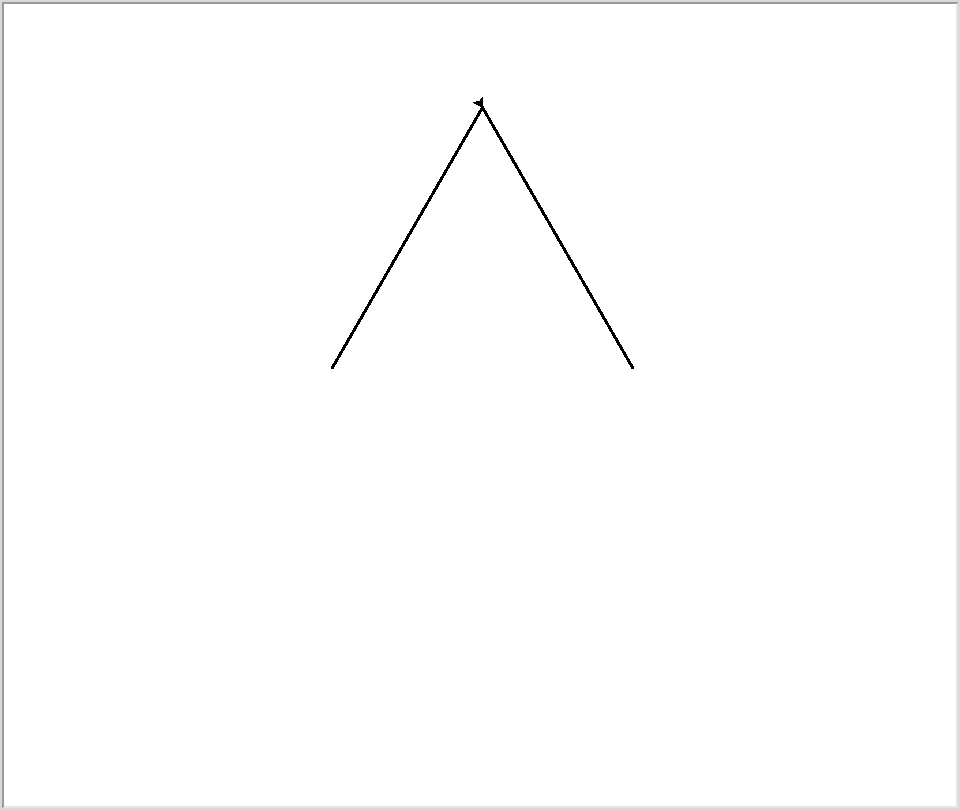
\includegraphics[scale=\myscale,scale=0.14]{ecran_tortue_arbre1}\quad 
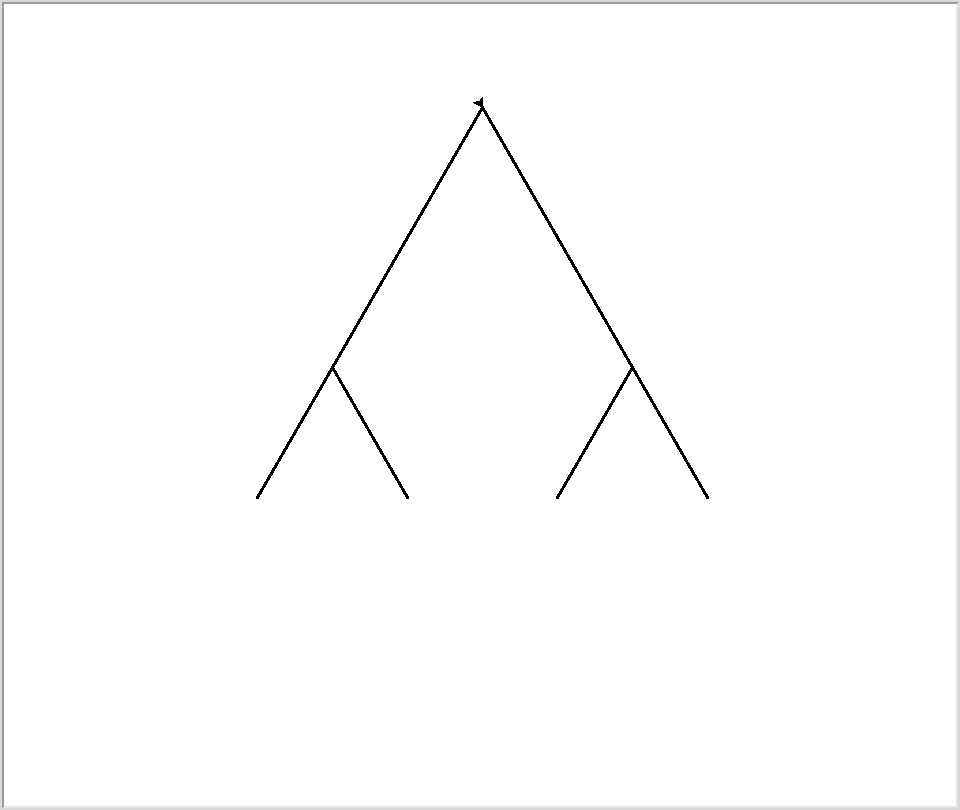
\includegraphics[scale=\myscale,scale=0.14]{ecran_tortue_arbre2}\quad
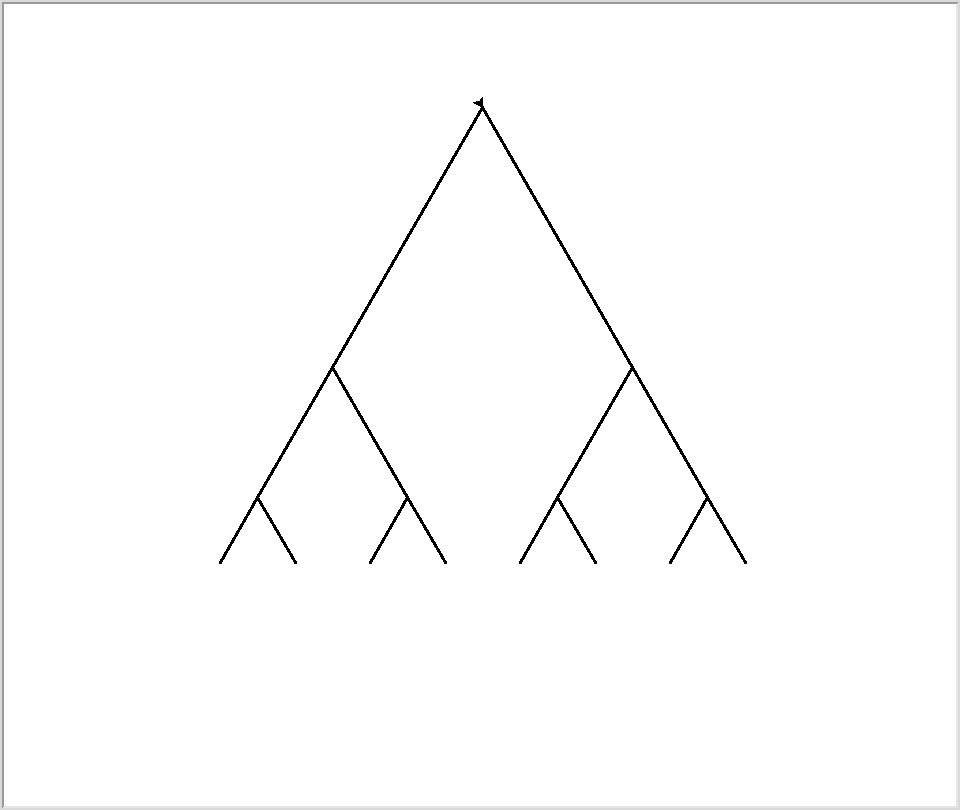
\includegraphics[scale=\myscale,scale=0.14]{ecran_tortue_arbre3}

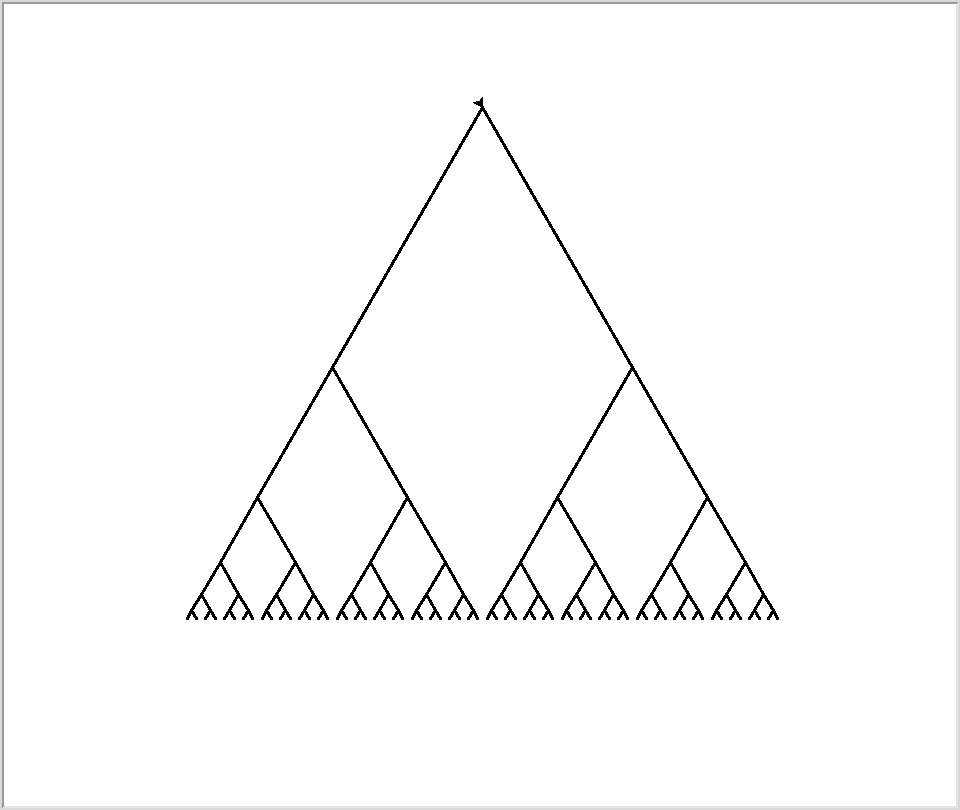
\includegraphics[scale=\myscale,scale=0.25]{ecran_tortue_arbre6}
\end{center}

  \item \textbf{Triangle de Sierpinski.}
  \index{fractale!triangle de Sierpinski}
  
  Trace les différentes étapes qui conduisent au triangle de Sierpinski par une fonction récursive \ci{triangle(l,n)} ($\ell$ est un paramètre de longueur, $n$ est un paramètre de profondeur).
  
   Voici les dessins pour $n=1$, $n=2$, $n=3$ et $n=6$.
  
  \begin{center}
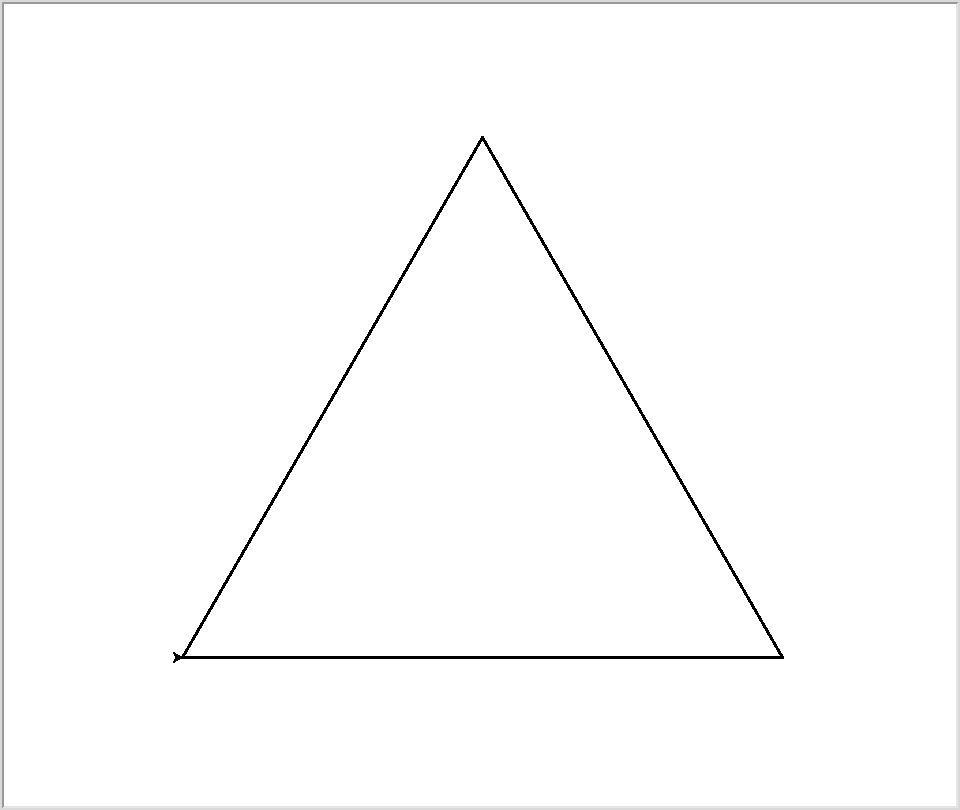
\includegraphics[scale=\myscale,scale=0.14]{ecran_tortue_sierp1}\quad 
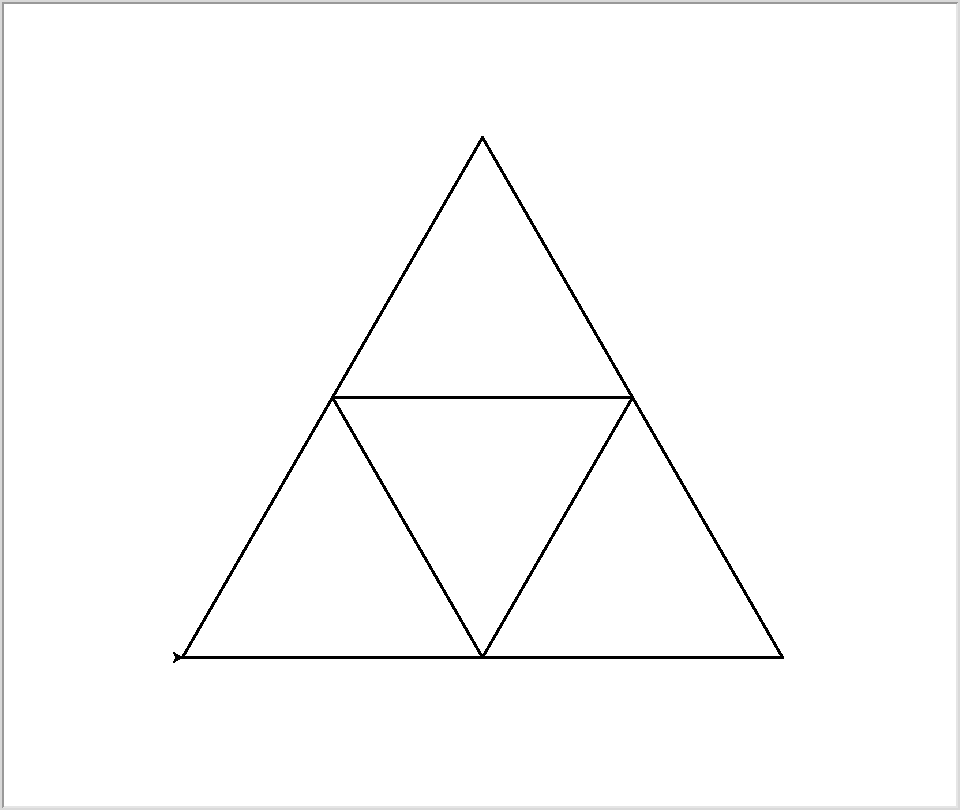
\includegraphics[scale=\myscale,scale=0.14]{ecran_tortue_sierp2}\quad
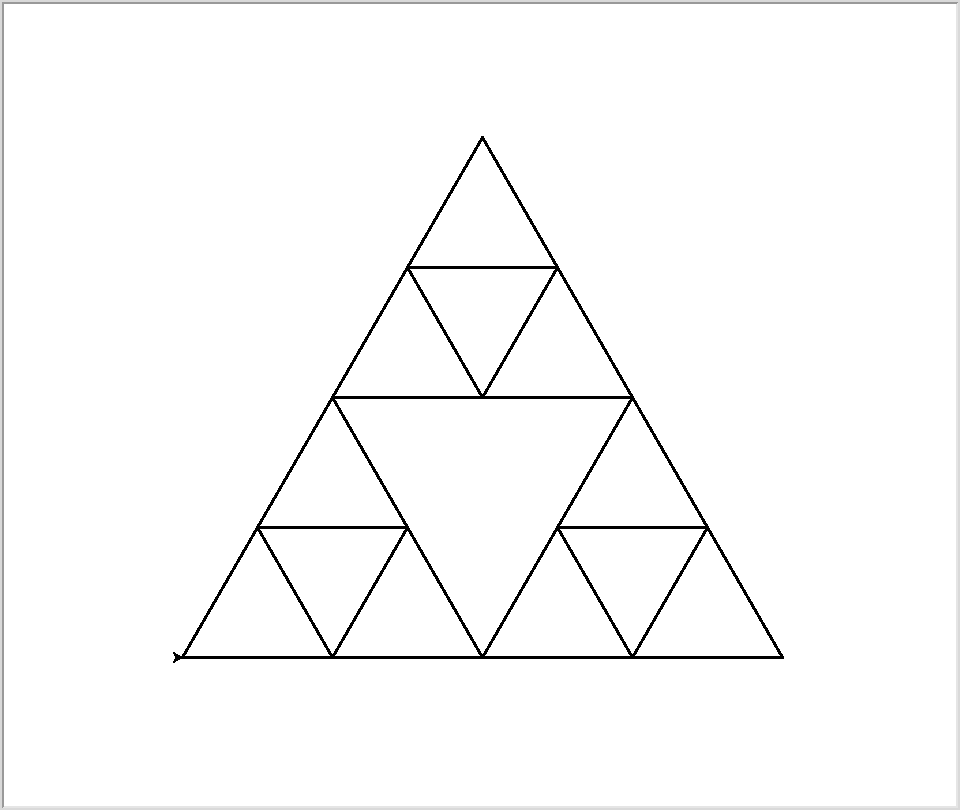
\includegraphics[scale=\myscale,scale=0.14]{ecran_tortue_sierp3}

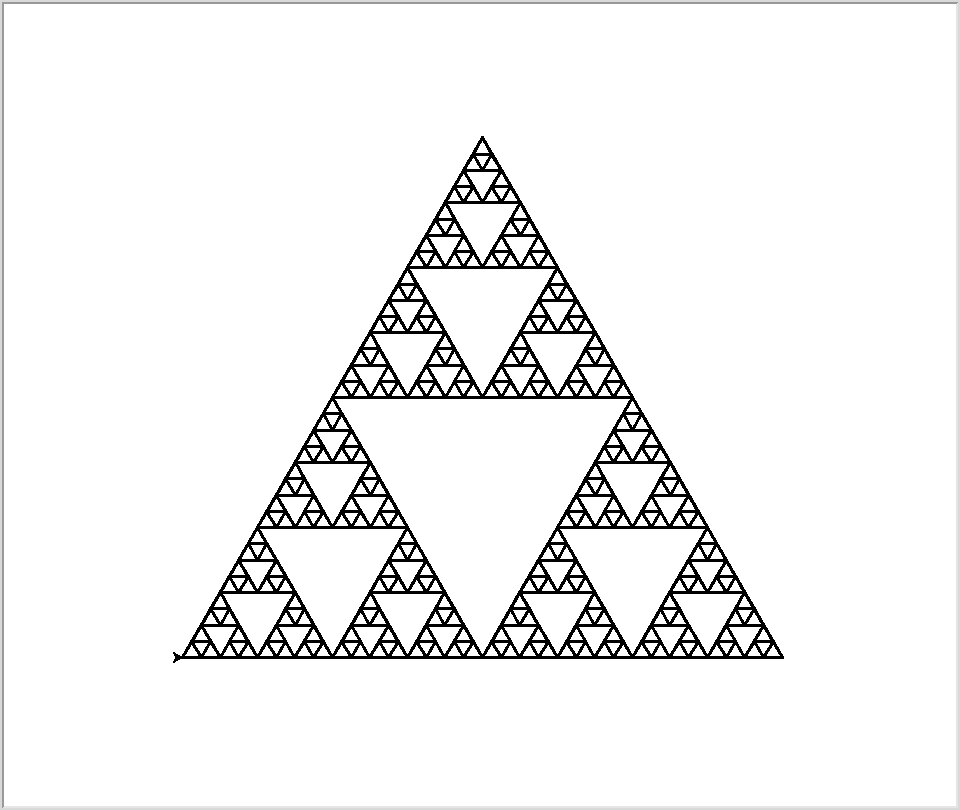
\includegraphics[scale=\myscale,scale=0.25]{ecran_tortue_sierp6}
\end{center}

Le principe récursif est le suivant :
\begin{itemize}
  \item Si $n=0$ ne rien faire.
  \item Sinon répéter trois fois :
  \begin{itemize}
    \item faire un appel récursif \ci{triangle(l/2,n-1)}, 
    \item avancer de $\ell$ pas,
    \item tourner de $120$ degrés.
  \end{itemize}
\end{itemize}


  \item \textbf{Courbe de Hilbert.}
  \index{fractale!courbe de Hilbert}
  
  Trace les premiers pas de la courbe de Hilbert à l'aide d'une fonction récursive
  \ci{hilbert(angle,n)}. 
  
  Le tracé récursif se fait selon le principe expliqué ci-dessous, $\ell$ est une longueur fixée à l'avance, $\theta$ est l'angle qui vaut $\pm 90$ degrés, $n$ est l'ordre du tracé.
  
\begin{itemize}
  \item Si $n=0$ ne rien faire.
  \item Sinon :
  \begin{itemize}
    \item tourner à gauche de $-\theta$,
    \item faire un appel récursif avec comme paramètres $-\theta$ et l'ordre $n-1$,
    \item avancer de la longueur $\ell$,
    \item tourner à gauche de $+\theta$,
    \item faire un appel récursif avec comme paramètres $+\theta$ et l'ordre $n-1$,
    \item avancer de la longueur $\ell$,
    \item faire un appel récursif avec comme paramètres $+\theta$ et l'ordre $n-1$,
    \item tourner à gauche de $+\theta$, 
    \item avancer de la longueur $\ell$,   
    \item faire un appel récursif avec comme paramètres $-\theta$ et l'ordre $n-1$,                
    \item tourner à gauche de $-\theta$.
  \end{itemize}
\end{itemize}
  
  
  Voici les dessins pour l'angle initial valant $\theta = +90$ degré et des ordres $n$ allant de $1$ à $6$.
  
   \begin{center}
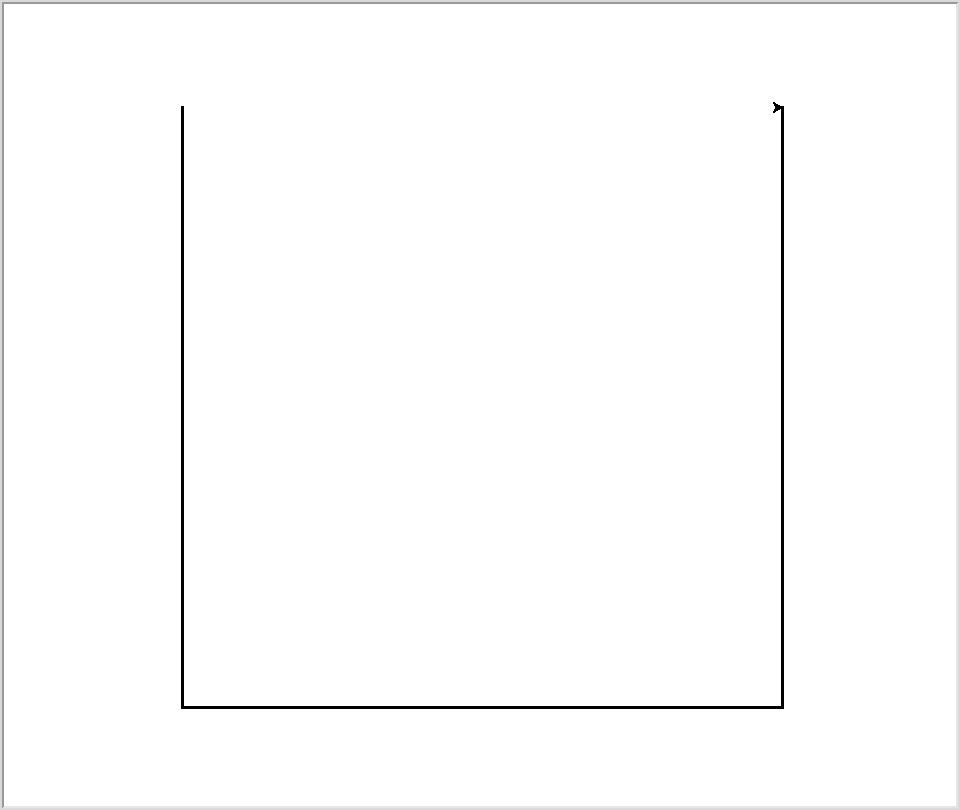
\includegraphics[scale=\myscale,scale=0.14]{ecran_tortue_hilbert1}\quad 
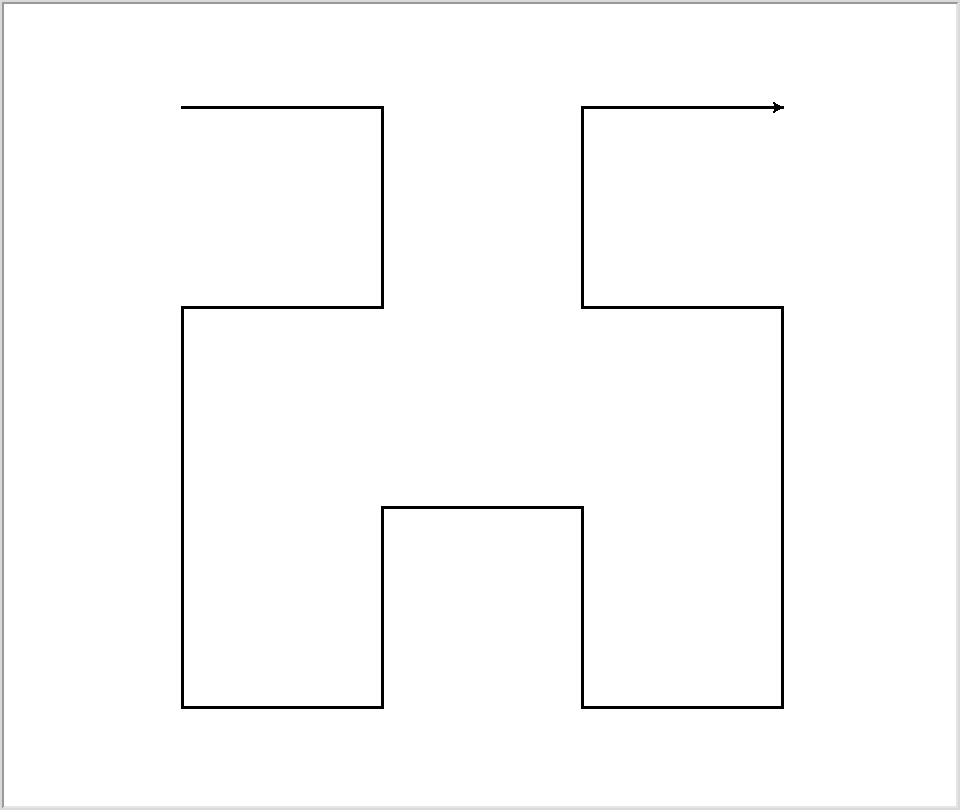
\includegraphics[scale=\myscale,scale=0.14]{ecran_tortue_hilbert2}\quad
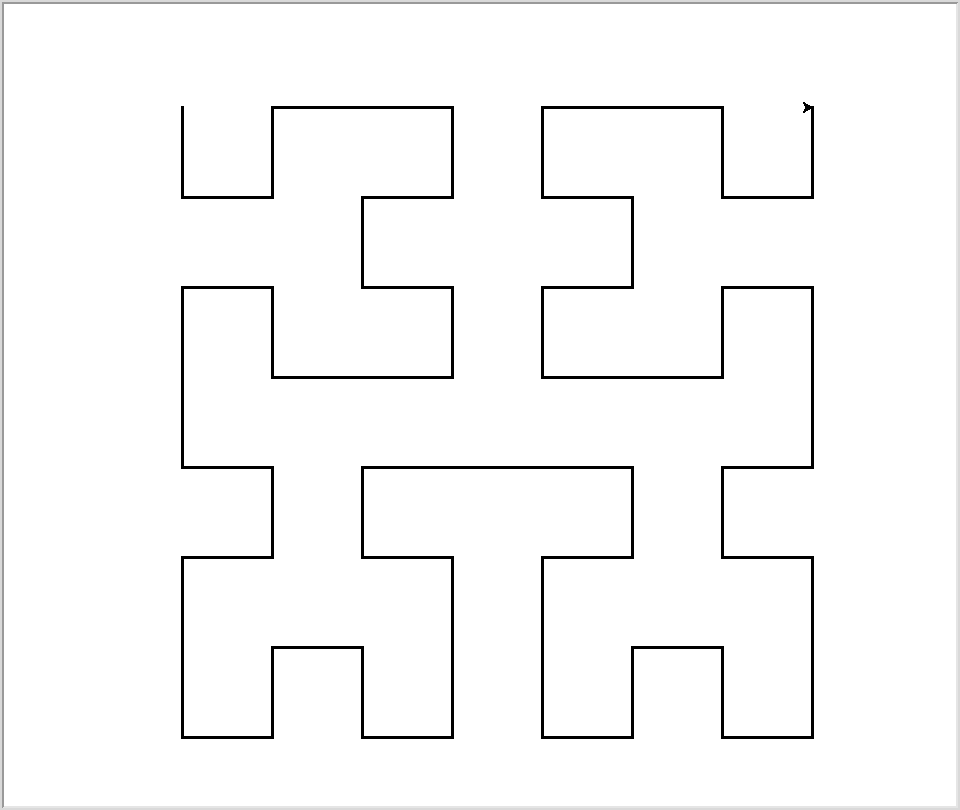
\includegraphics[scale=\myscale,scale=0.14]{ecran_tortue_hilbert3}

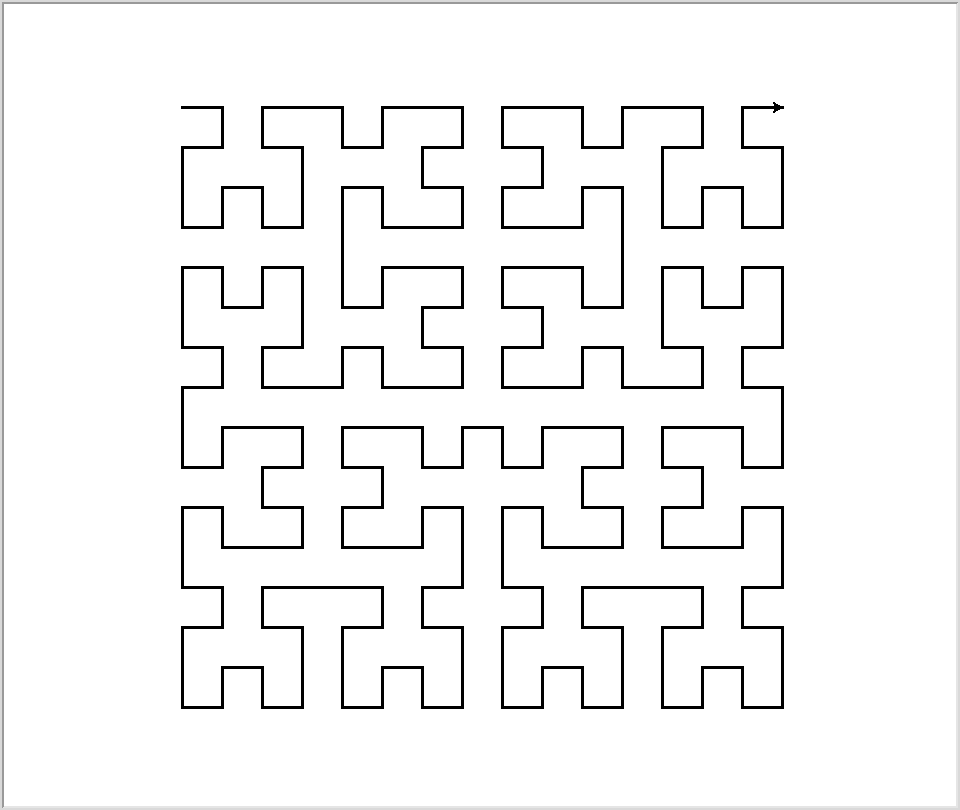
\includegraphics[scale=\myscale,scale=0.14]{ecran_tortue_hilbert4}\quad
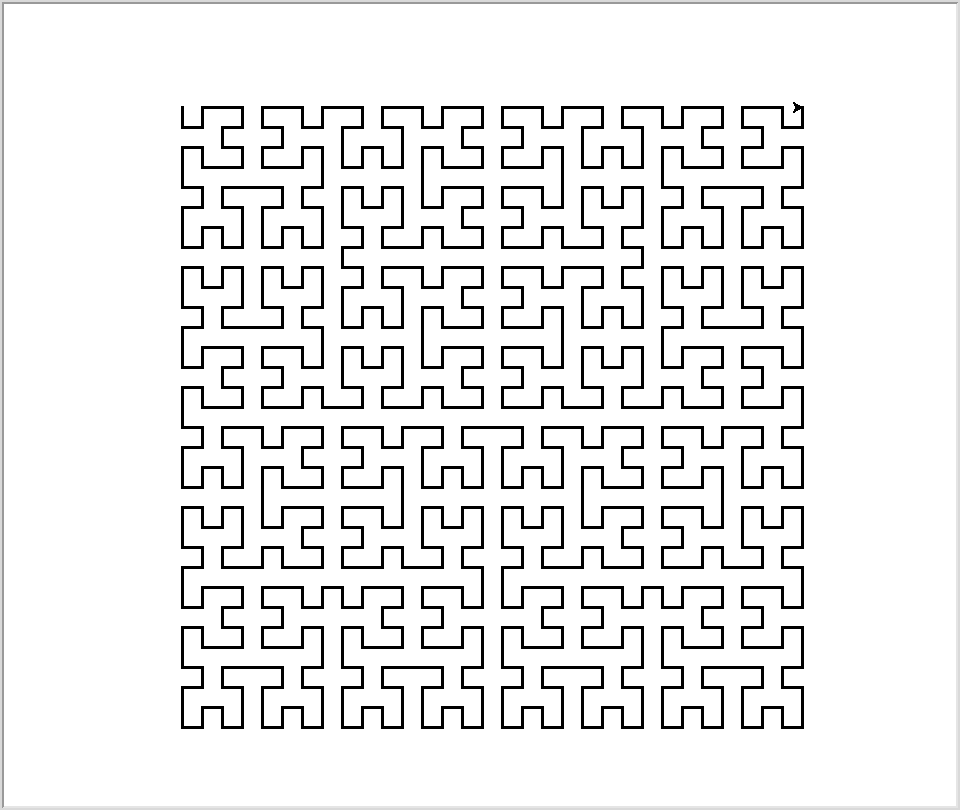
\includegraphics[scale=\myscale,scale=0.14]{ecran_tortue_hilbert5}\quad
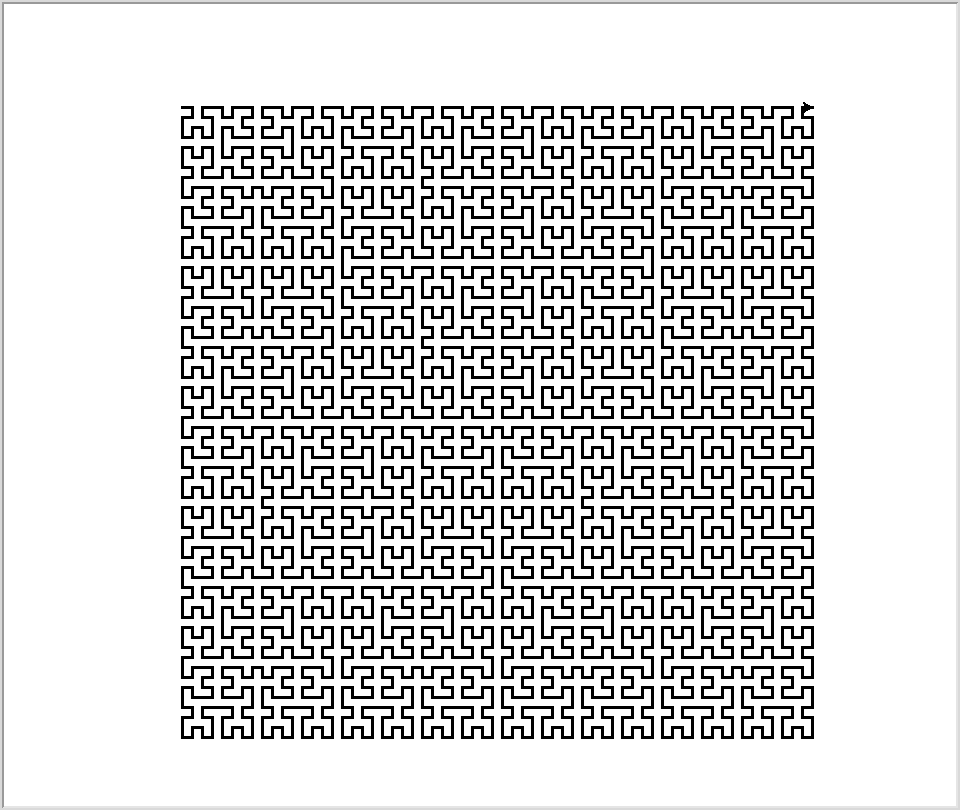
\includegraphics[scale=\myscale,scale=0.14]{ecran_tortue_hilbert6}
\end{center} 
  
  \item \textbf{Fractale aléatoire.}
  
  Programme une fonction récursive \ci{fractale_cercle(l,n)} qui contient une part d'aléatoire. La fonction dessine un quart de cercle, puis décide au hasard (une chance sur deux par exemple) si elle trace un plus petit cercle par un appel récursif, ensuite elle continue avec le tracé d'un quart du cercle initial et décide alors de tracer éventuellement un plus petit cercle\ldots 
  
   Voici des dessins pour $n=1$, $n=2$, $n=3$ et $n=4$. Bien sûr d'une fois sur l'autre le dessin change au hasard.
  
  \begin{center}
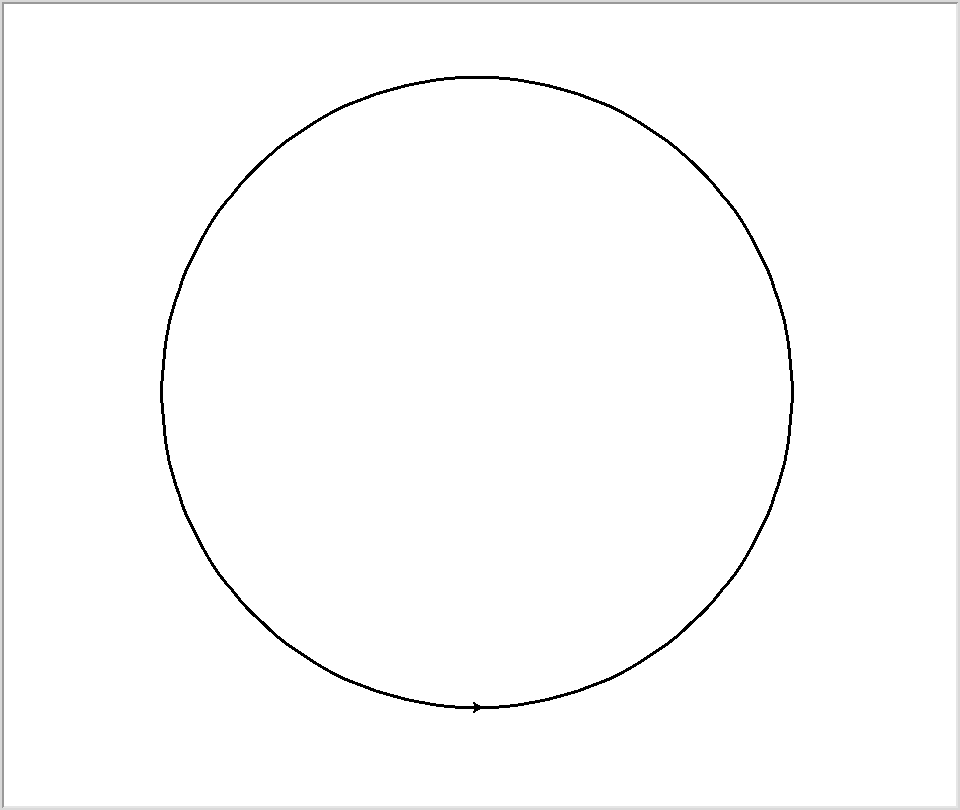
\includegraphics[scale=\myscale,scale=0.14]{ecran_tortue_cercle1}\quad 
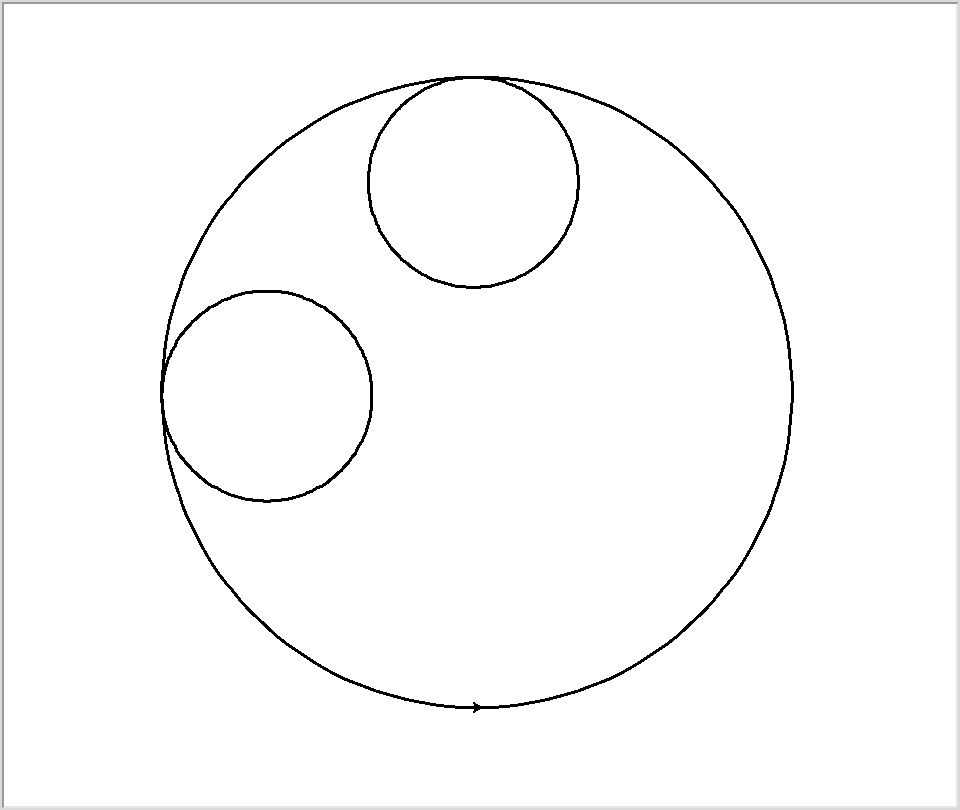
\includegraphics[scale=\myscale,scale=0.14]{ecran_tortue_cercle2}\quad
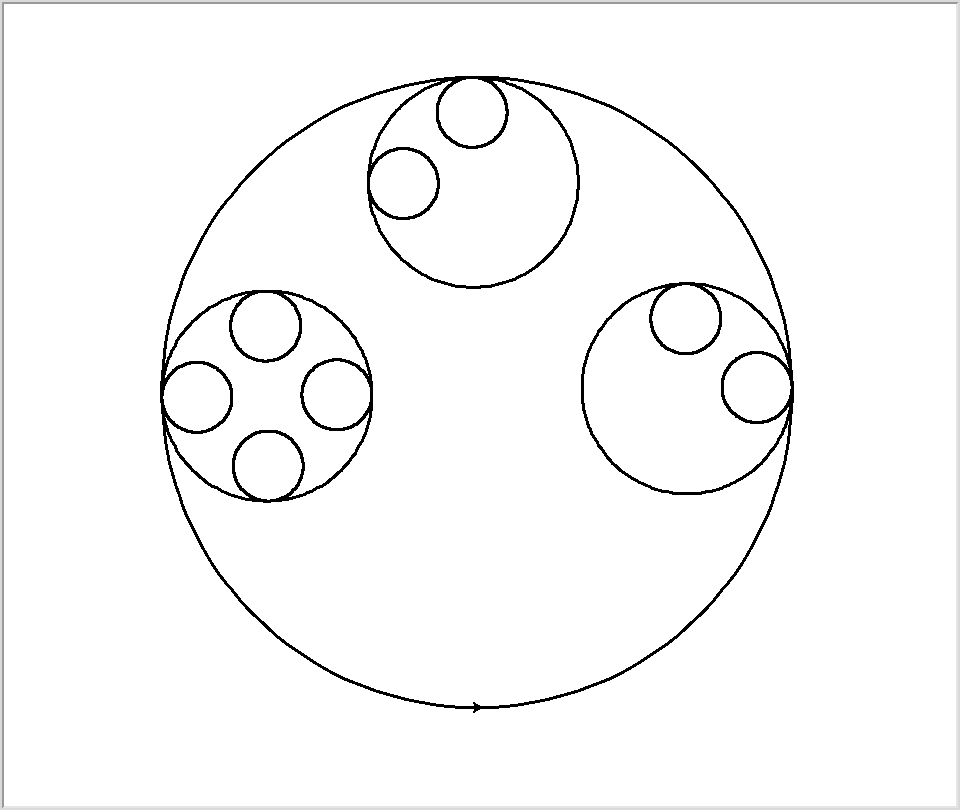
\includegraphics[scale=\myscale,scale=0.14]{ecran_tortue_cercle3}

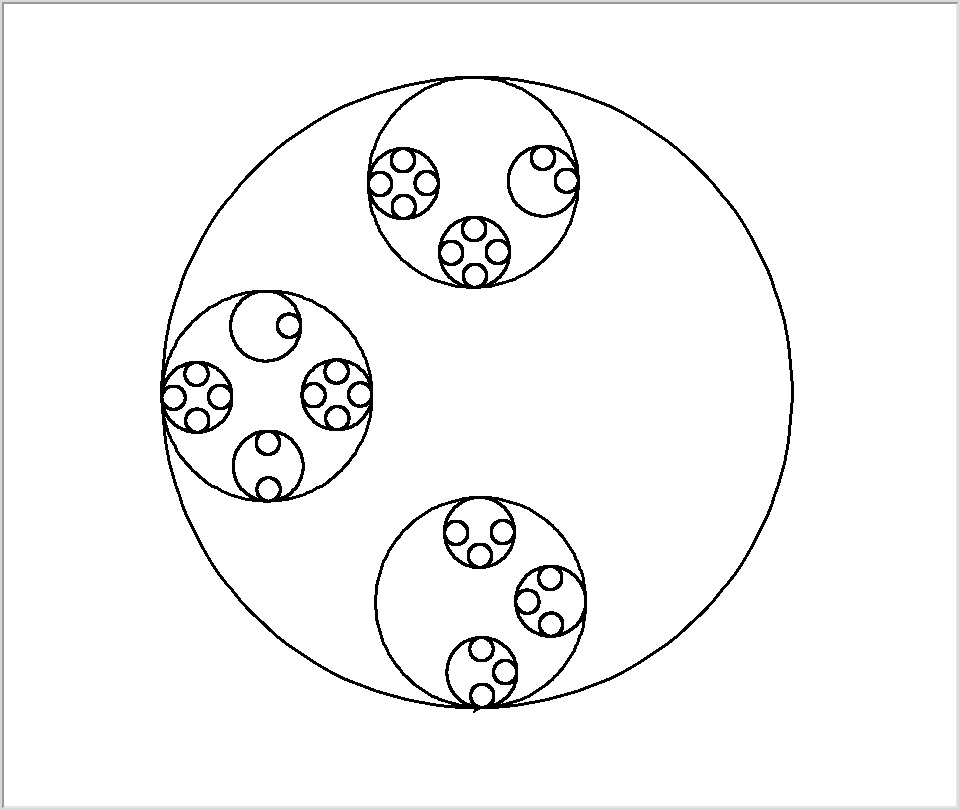
\includegraphics[scale=\myscale,scale=0.25]{ecran_tortue_cercle4}
\end{center}  
  
\end{enumerate}
 
\end{activite}


\end{document}
